\documentclass[a4paper]{article}
\usepackage[french]{babel}
\usepackage[utf8]{inputenc}
\usepackage[T1]{fontenc}
\usepackage{todonotes}
\usepackage{graphicx}
\usepackage{subcaption}
\usepackage{amssymb} % nécessaire pour \mathbb
\usepackage{mathtools}
\usepackage{csquotes}
\usepackage[style=ieee]{biblatex}
\addbibresource{ref.bib}
\bibliography{ref.bib}
\usepackage{hyperref}

% If you use the hyperref package, please uncomment the following line
% to display URLs in blue roman font according to Springer's eBook style:
\renewcommand\UrlFont{\color{blue}\rmfamily}

\title{Rapport projet TLNL}
\author{Leader : Adrien ZABBAN \\ Follower : Yanis LABEYRIE}
\date{05 novembre 2023}

\begin{document}
\maketitle


\section{Introduction}

Le but de ce projet est de coder un modèle de langage basé sur un réseau de neurone multicouche. Ce modèle de langage devra permettre 
de prédire le mot suivant à partir d'un contexte, qui est un ensemble de mots précédent le mot à prédire. 

Pour faire cela, on utilise des embeddings. Le principe est d'associer à chaque mot un vecteur dans un espace latent de tels sorte que 
deux mots similaires (en termes de sens) ont des vecteurs proches (avec une distance euclidienne), et deux mots totalement différents 
sont très loin. Cela permet de projeter les mots dans un espace latent pour pouvoir travailler plus efficacement sur ces mots. 
On note $e$ la dimension de cette espace.

Dans un premier temps, on utilisera les embeddings des mots appris par l'algorithme Word2Vect~\cite{mikolov2013efficient} 
(modèle nommé \textit{FROZEN}). Par la suite, nous tenterons d'améliorer le modèle en lui permettant d'apprendre ses propres 
embeddings à partir d'embeddings aléatoire (modèle nommé \textit{SCRATCH}), ou directement les embeddings appris de Word2Vect 
(modèle nommé \textit{ADAPT}).


\section{Modèle \textit{FROZEN}}

Nous avons implémenté le perceptron multicouche comme modèle de langage de base. Celui-ci est composé d'une couche d'entrée qui 
prenant un vecteur de dimension $k \times e$ représentant les embeddings de $k$ mots concaténés. Une couche de neurone cachée dont 
nous avons choisi de faire varier le nombre de neurone noté $h$, suivit d'une fonction ReLU~\cite{DBLP:journals/corr/abs-1803-08375}. 
Puis une deuxième couche de neurones suivit d'un softmax retournant un vecteur de taille $V$, le nombre de mots appris. 
La Figure~\ref{fig:model1} représente ce modèle.

\subsection{Formalisme mathématiques}
En notant, $W \in \mathcal{M}_{k \times e, h_1}(\mathbb{R})$, et $U \in \mathcal{M}_{h, V}(\mathbb{R})$ les matrices de poids, 
$(b_1,b_2) \in \mathbb{R}^{h} \times \mathbb{R}^{V}$ les biais, $X \in \mathbb{R}^{k \times e}$ le vecteur d'entrée, 
l'équation~\eqref{eq:model1} donne la fonction de sortie $F(X) \in \mathbb{R}^{V}$ du modèle. 


Après plusieurs essais, nous avons choisie de prendre: $k=3$, $e=100$, $h_1=256$. Et dans nos données d'entraînement, on avait un 
vocabulaire contenant: $V=2908$ mots distincts. Avec ces hyperparamètres, nous avons dans ce modèle $824412$ paramètres apprenables.
% temps d'apprentisage pour 10 epochs: 13min

\begin{flalign}
    & F(x)=softmax(U(ReLU(WX+b_1))+b_2) \label{eq:model1} &
\end{flalign}

\begin{figure}
    \centering
    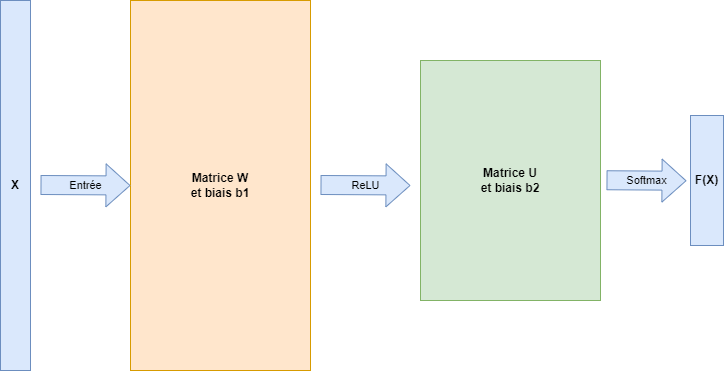
\includegraphics[width=0.60\linewidth]{model1.png}
    \caption{Modèle: \textit{FROZEN}}
    \label{fig:model1}
\end{figure}

Pour entraîner ce modèle, nous avons comparer notre sortie au mot à prédire dans le format One-hot encoding
\footnote{Le format One-hot encoding est un encodage des indices en un vecteur d'une taille du nombre d'indice possible tel que 
ce vecteur possède des 0 partout sauf à l'indice en question qui possède un 1.}, et nous appliquons le calcule de la fonction de 
coût: cross-entropy. 
On avons utilisé Adam~\cite{kingma2014adam} pour optimiser les paramètres avec un learning rate de $0.01$ pour les 5 premières 
époques et $0.001$ pour les suivantes.

\subsection{Métriques}
Nous avons par ailleurs décidé d'évaluer ce réseau à l'aide de plusieurs métriques comme l'accuracy, la perplexité, le $f_1$-score 
et la métrique "top~$k$"\footnote{La métrique "top-$k$" évalue un modèle en comptant combien de prédictions correctes il fait parmi 
les $k$ premières prédictions les plus probables. Attention ici $k$ n'est pas le nombre de mots dans le contexte!} (avec $k=5$), 
voir~\cite{DBLP:journals/corr/LiuDLZ15}.

\subsection{Résultats}

Sur la Figure~\ref{subfig:result model 1}, on voit les courbes d'apprentissage. Les valeurs des métriques sur les données 
d'entraînement sont en bleue, sur les données de validations sont en orange.

On constate d'après les courbes que le modèle apprend très vite (les courbes atteignent un plateau en quasiment 2 epochs). Ceci 
est du au fait que les embeddings du modèle sont déjà appris. On observe par ailleurs que le modèle n'overfit pas car il n'y a pas 
de décalage important entres les valeurs de métrique d'entraînement et de validation à la fin de l'entraînement. Le modèle se 
stabilise à la fin de l'entraînement avec les métriques de validation présenté dans la Table~\ref{tab:metriques model1}.


\begin{table}
    \centering
    \begin{tabular}{|c|c|c|c|c|}
        \hline
        métriques & accuracy  & top $k$  & perplexité  & $f_1$ score \\
        \hline
        modèle \textit{FROZEN} & 0.19 & 0.34  & 144 & 9.6e-4 \\
        \hline
    \end{tabular}
    \caption{Meilleures métriques de validation obtenues en fin d'apprentissage du modèle \textit{FROZEN}.}
    \label{tab:metriques model1}
\end{table}


\begin{figure}[ht]
  \centering
  \begin{subfigure}{0.47\textwidth}
    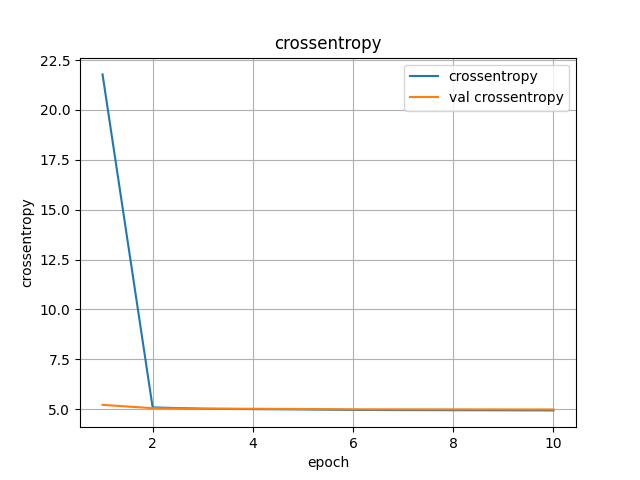
\includegraphics[width=\linewidth]{../logs/word2vect/crossentropy.png}
    \caption{Cross Entropy Loss (Lower is Better)}
  \end{subfigure}
  \hfill
  \begin{subfigure}{0.47\textwidth}
    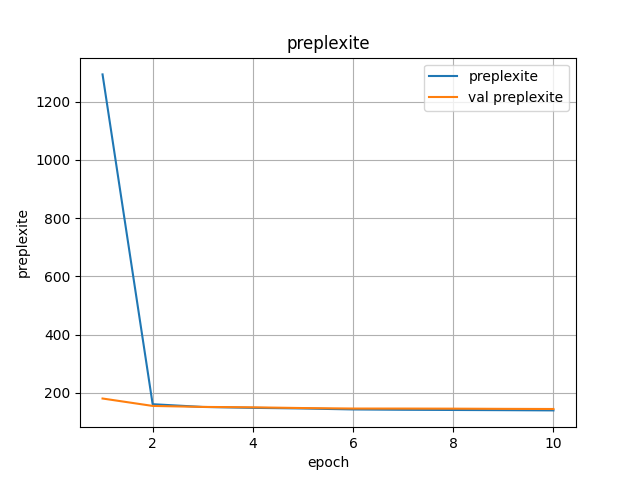
\includegraphics[width=\linewidth]{../logs/word2vect/preplexite.png}
    \caption{perplexité (Lower is Better)}
  \end{subfigure}

  \begin{subfigure}{0.47\textwidth}
    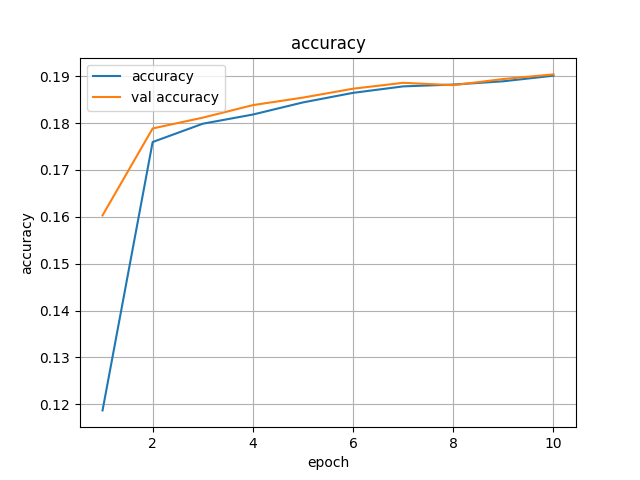
\includegraphics[width=\linewidth]{../logs/word2vect/accuracy.png}
    \caption{Accuracy (Higher is Better)}
  \end{subfigure}
  \hfill
  \begin{subfigure}{0.47\textwidth}
    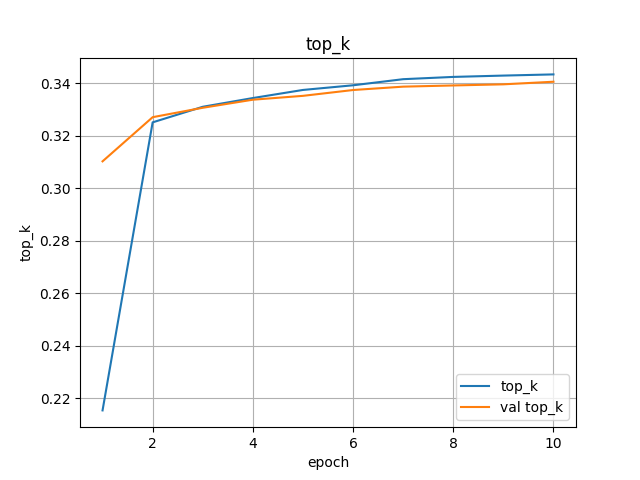
\includegraphics[width=\linewidth]{../logs/word2vect/top_k.png}
    \caption{top k, avec k=5 (Higher is Better)}
  \end{subfigure}
  \caption{Entraînement du modèle \textit{FROZEN}}
  \label{subfig:result model 1}
\end{figure}


\section{Apprentissage automatique des embeddings par le modèle de langage: modèle \textit{SCRATCH}}

\subsection{Description}

Cette première piste que nous avons exploré consiste à se dire que notre modèle d'embeddings pré-entraîné n'est pas forcément 
pertinent pour la tâche de prédiction du mot suivant d'une phrase. L'idée est donc de considérer que la matrice d'embeddings 
peut-être apprise par le modèle de langage et que la matrice apprise sera plus pertinente qu'une matrice apprise séparément pour 
résoudre la tâche. On va donc considérer que les paramètres de la matrice sont des paramètres apprenables du modèle de langage et 
donc étendre jusqu'à eux l'algorithme de rétro-propagation du gradient.

\subsection{Mise en \oe uvre}

Il a fallut adapter un peu notre code car avant pour avoir l'embedding d'un mot $i$, on utilisé $E[i]$, où 
$E \in \mathcal{M}_{V, e}(\mathbb{R})$ est la matrice d'embedding. Cependant, cette opération n'est pas dérivable, donc il a 
fallut transformer le mot $i$ en un vecteur $x \in \mathbb{R}^V$ one-hot, et faire $x \times E$ pour obtenir l'embedding du 
mots $i$, qui cette fois ci, est une opération dérivable. 
Une fois cette adaptation faite, on a rajouté cette opération dans notre modèle et nous obtenons donc un nouveau modèle illustré 
par la Figure~\ref{fig:model2}, et donné par l'équation~\eqref{eq:model2}.


\begin{flalign}
    & F(x)=softmax(U(ReLU(W\tilde{X}+b_1))+b_2) \label{eq:model2} & \\
    & \quad \text{où } \tilde{X}=flatten(XE)  \quad \text{et} \quad X \in \mathcal{M}_{k, V}(\mathbb{R}) \notag &
\end{flalign}

\begin{figure}
    \centering
    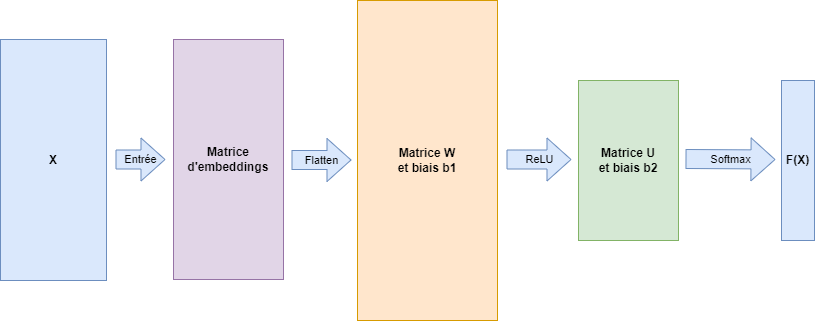
\includegraphics[width=0.60\linewidth]{model2.png}
    \caption{Modèle: \textit{SCRATCH} avec l'apprentissage des embeddings}
    \label{fig:model2}
\end{figure}


\subsection{Résultats}


On remarque, sur la Figure~\ref{subfig:result model 2}, tout d'abord que l'apprentissage à la fois du modèle et des embeddings est plus 
long car l'ensemble (modèle plus matrice d'embedding) possède un plus grand nombre de paramètres ($1115212$ contre $824412$ pour le 
modèle \textit{FROZEN}) qui nécessitent donc plus d'epochs que \textit{FROZEN} pour être actualisés.

On obtient en terme de métriques de validation, des résultats semblables au modèle précèdent. Cela s'explique par le fait que, bien 
qu'on apprenne par rétro-propagation les embeddings et que donc on s'attend à une meilleur qualité de résultat, cela est compensé par 
le fait que l'apprentissage se fait à partir de 0 et on commence donc l'apprentissage avec des résultats aléatoires.

A la fin de l'apprentissage, nous obtenons les métriques de validation suivantes, comme on peut le voir dans la 
Table~\ref{tab:metriques model2}.


\begin{figure}[ht]
  \centering
  \begin{subfigure}{0.47\textwidth}
    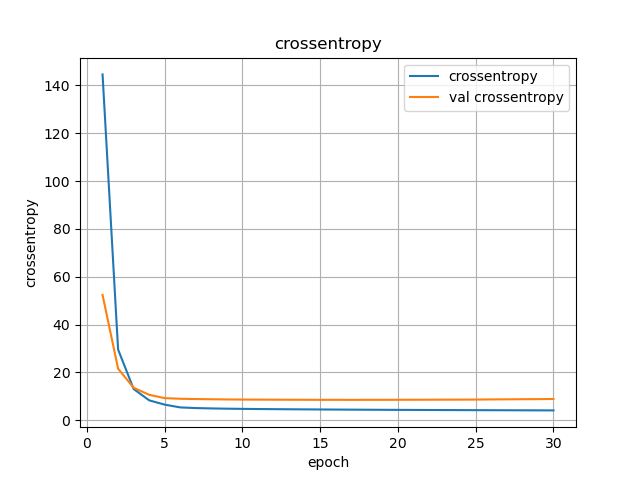
\includegraphics[width=\linewidth]{../logs/learnfromscratch_1/crossentropy.png}
    \caption{Cross Entropy Loss (Lower is Better)}
  \end{subfigure}
  \hfill
  \begin{subfigure}{0.47\textwidth}
    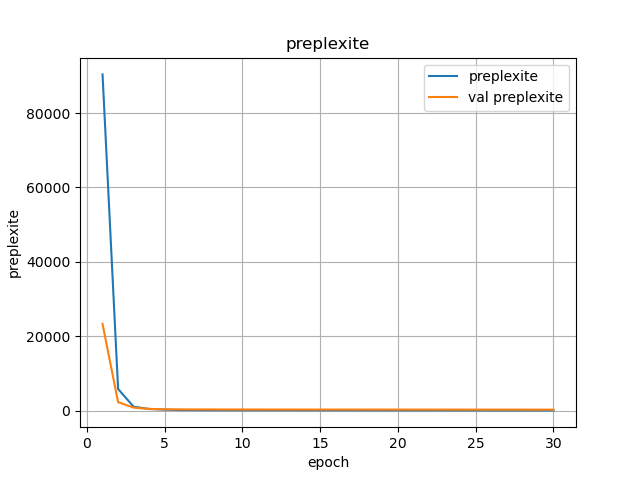
\includegraphics[width=\linewidth]{../logs/learnfromscratch_1/preplexite.png}
    \caption{perplexité (Lower is Better)}
  \end{subfigure}

  \begin{subfigure}{0.47\textwidth}
    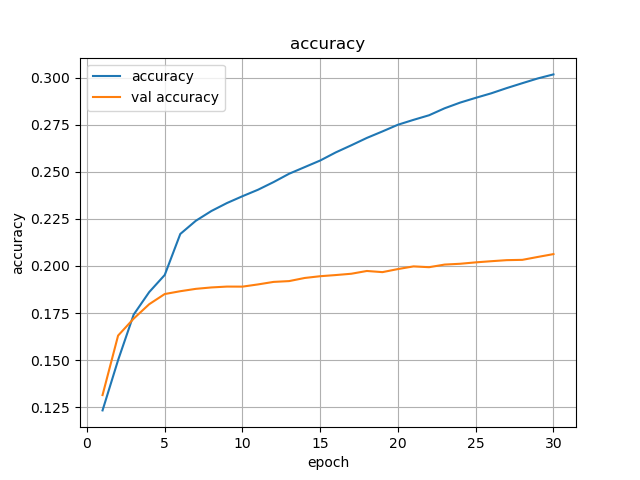
\includegraphics[width=\linewidth]{../logs/learnfromscratch_1/accuracy.png}
    \caption{Accuracy (Higher is Better)}
  \end{subfigure}
  \hfill
  \begin{subfigure}{0.47\textwidth}
    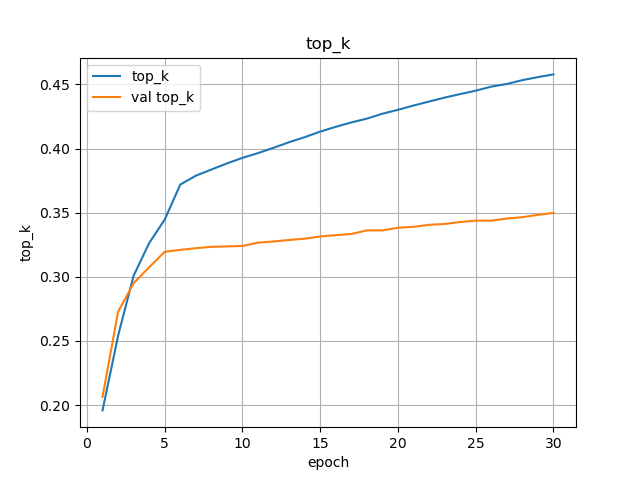
\includegraphics[width=\linewidth]{../logs/learnfromscratch_1/top_k.png}
    \caption{top k, avec k=5 (Higher is Better)}
  \end{subfigure}
  \caption{Entraînement du modèle \textit{SCRATCH}}
  \label{subfig:result model 2}
\end{figure}

\begin{table}
    \centering
    \begin{tabular}{|c|c|c|c|c|}
        \hline
        modèle & accuracy  & top $k$  & perplexité  & $f_1$ score \\
        \hline
        \textit{FROZEN} & 0.19 & 0.34  & 144 & 9.6e-4 \\
        \hline
        \textit{SCRATCH} & 0.195 & 0.333  & 280.37 & 1.27e-3 \\
        \hline
    \end{tabular}
    \caption{Meilleures métriques de validation obtenues en fin d'apprentissage des modèles \textit{FROZEN} et \textit{SCRATCH}.}
    \label{tab:metriques model2}
\end{table}


\section{Apprentissage des embeddings à partir de l'algorithme Word2Vect: modèle \textit{ADAPT}.}

\subsection{Description}

Dans cette partie, nous allons tenter d'améliorer la performance et surtout la vitesse d'apprentissage. Au lieu,
d'initialiser la matrice d'embedding aléatoirement comme dans la partie précédente, nous allons initialiser cette 
matrice à partir des embeddings déjà appris avec l'algorithme Word2Vect. En procédant comme cela, nous allons pouvoir
continuer d'apprendre ces embeddings pour coller au mieux à notre tâche de prédiction.

\subsection{Mise en \oe uvre}

La mise en \oe uvre de cette partie n'a pas été très compliqué à implémenter car le modèle est le même que celui de 
\textit{SCRATCH}, voir Figure~\ref{fig:model2}. Il nous a donc suffit de récupérer la matrice d'embedding apprise et de 
la copier dans le modèle lors de son initialisation.

\subsection{Résultats}

On constate immédiatement, avec la Figure~\ref{subfig:result model 3}, que l'apprentissage est bien plus rapide dans le cas où on 
initialise les embeddings avec Word2Vect par rapport au cas où on les initialise aléatoirement. Cela s'explique par le fait que 
contrairement au modèle précédent, le modèle a déjà des embeddings valides aux début de l'apprentissage qu'il peut par la suite 
perfectionner.

Notre hypothèse était que initialiser les embeddings avec Word2Vect puis les modifier au cours de l'apprentissage permettrait 
d'obtenir de meilleurs performances que celles du modèle où les embeddings sont gelés pendant l'apprentissage. 


\begin{figure}[ht]
  \centering
  \begin{subfigure}{0.47\textwidth}
    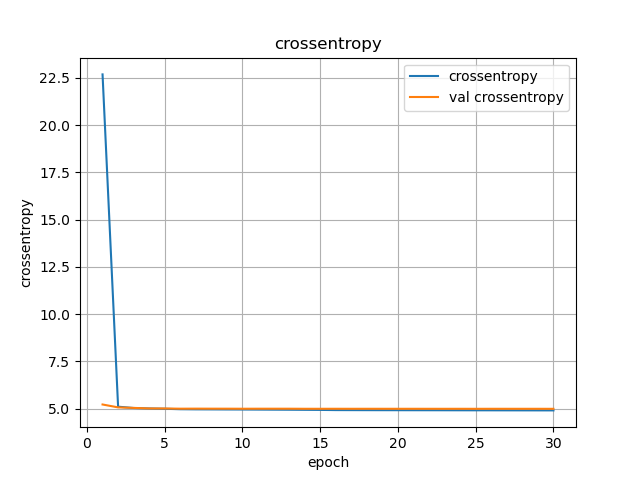
\includegraphics[width=\linewidth]{../logs/learnfromword2vect_0/crossentropy.png}
    \caption{Cross Entropy Loss (Lower is Better)}
  \end{subfigure}
  \hfill
  \begin{subfigure}{0.47\textwidth}
    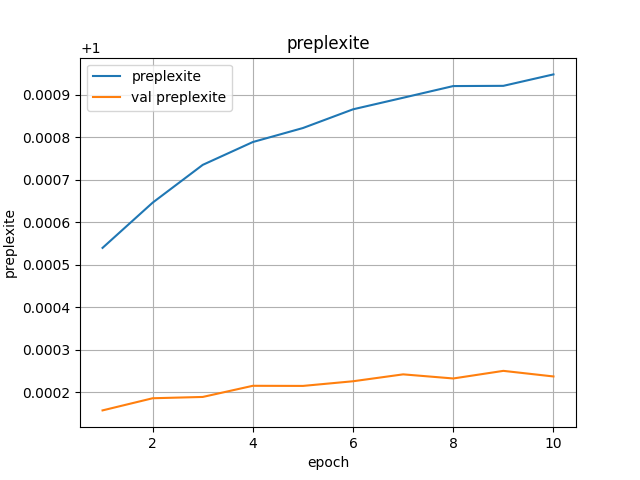
\includegraphics[width=\linewidth]{../logs/learnfromword2vect_0/preplexite.png}
    \caption{perplexité (Lower is Better)}
  \end{subfigure}

  \begin{subfigure}{0.47\textwidth}
    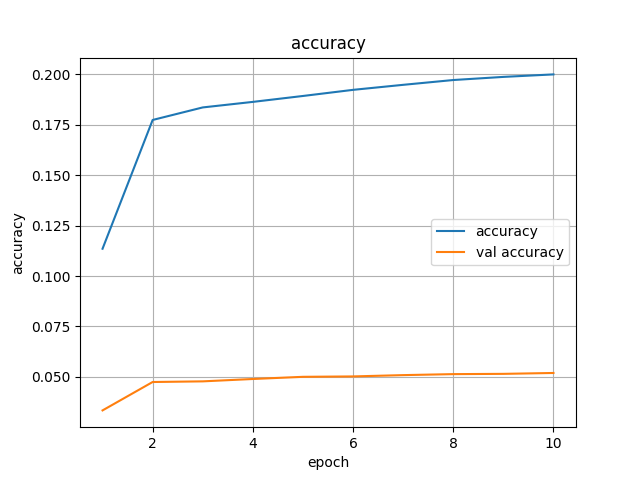
\includegraphics[width=\linewidth]{../logs/learnfromword2vect_0/accuracy.png}
    \caption{Accuracy (Higher is Better)}
  \end{subfigure}
  \hfill
  \begin{subfigure}{0.47\textwidth}
    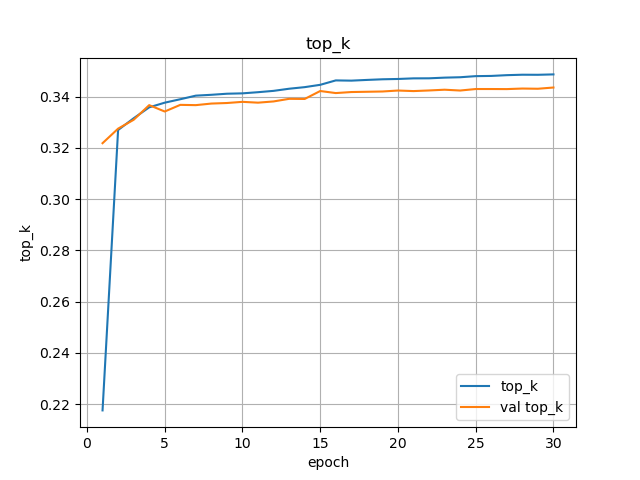
\includegraphics[width=\linewidth]{../logs/learnfromword2vect_0/top_k.png}
    \caption{top k, avec k=5 (Higher is Better)}
  \end{subfigure}
  \caption{Entraînement du modèle \textit{ADAPT}}
  \label{subfig:result model 3}
\end{figure}


\section{Conclusions et perspectives}

\subsection{Performance}

Après avoir entraîné ces trois modèles et pris les poids qui minimise la loss de validation, nous avons ensuite passé ces modèles dans 
une base de données de teste\footnote{La base de données est bien sûr disjointe de celles de l'entraînement et de validation, mais toujours
tirée du corpus du \textit{Compte de Monté-Cristo} d'Alexendre Dumas.}. La Table~\ref{tab:test} présente les résultats des modèles sur 
différentes métriques. On voir que les 3 modèles ont une accuracy et une métrique top~$k$ similaires. Cependant, le modèle \textit{SCRATCH} 
est très mauvais sur la Cross Entropy et la perplexité (par rapport aux autres modèles). Il est aussi étonnant de constater que le modèle
\textit{FROZEN} et \textit{ADAPT} ont des résultats similaires. Cela sigifie que les embeddings appris par Word2Vect correspondes à cette tâche.
Dans ce cas, les embeddings obtenues avec Word2Vect ont été appris sur le même corpus que l'entraînement des modèles. Nous pensons que si 
les embeddings aurait été appris sur un autre corpus, le modèle \textit{ADAPT} aurai pu se différencier par rapport au modèle \textit{FROZEN}.


\begin{table}[ht]
    \centering
    \begin{tabular}{|c|c|c|c|c|c|}
        \hline
        modèles & Cross Entropy & accuracy & top $k$ & $f_1$ score & perplexité \\
        \hline
        \textit{FROZEN} & $4.89$ &  $0.20$ & $0.35$ & $9.42e-4$ & $131$ \\
        \textit{SCRATCH} & $8.05$ &  $0.20$ & $0.35$ & $1.16e-3$ & $247$ \\
        \textit{ADAPT} & $4.90$ &  $0.20$ & $0.35$ & $8.86e-4$ & $130$ \\
        \hline
    \end{tabular}
    \caption{Résultat des différents modèles sur la base de données de teste.}
    \label{tab:test}
\end{table}

\subsection{Temps d'entraînement}

Il peut aussi être intéresant de regarder le temps d'entraînement des différents modèles, voir Table~\ref{tab:times}. Ces modèles ont été
entraîner sur un Windows 11 possèdant un intel i7 de 12ème génération et une carte graphique: Nvidia RTX 3050 modèle ordinateur portable.
On remarque sans surprise que l'entraînement le plus rapide est celui de \textit{FROZEN} car c'est le modèle qui a le moins de paramètres.
Il est très intéresant de voir que le modèle \textit{ADAPT} s'entraine beaucoup plus vite que le modèle \textit{SCRATCH}, alors que le
nombre de paramètres est le même. Notre hypothèse est que: \textit{mettre notre hypothèse}.
En comparant les résultats des modèles et leurs temps d'entraînement, on peut voir qu'il n'est pas rentable d'entraîner un modèle comme
celui de \textit{SCRATCH}, si l'on a déjà une partie pré-entraîné car cela prend beaucoup de temps et que l'on des performances 
plus faibles.

\begin{table}[ht]
    \centering
    \begin{tabular}{|c|c|c|c|}
        \hline
        modèles & \textit{FROZEN} & \textit{SCRATCH} & \textit{ADAPT} \\
        \hline
        temps (en s) & 360 & 1001 & 460 \\
        \hline
        nombre de paramètres & $800$k & $11$M & $11$M \\
        \hline
    \end{tabular}
    \caption{Comparaison du temps d'entraînement des différents modèles sur 10 epochs et nombre de paramètres apprenables des modèles.}
    \label{tab:times}
\end{table}

\subsection{Génération de texte}

\newpage

\printbibliography


\end{document}
